\chapter{Git history}
\label{ch:git_history}

The development lifecycle of the ClauseIQ system has been tracked using the Git distributed version control system and hosted on GitHub. This chapter documents the chronological progression of commits across the active development branch, reflecting the iterative evolution from initial exploratory data analysis through baseline machine learning, feature optimization, backend API hardening, and frontend user interface deployment.

\paragraph*{Repository overview}
The repository configuration and version control metadata for ClauseIQ are:
\begin{itemize}
    \item Repository URL: \url{https://github.com/Farhan-kalady/ClauseIQ.git}
    \item Active development branch: \texttt{feature/complete-clauseiq}
    \item Total development commits: 13 verified commits
    \item Tracking period: August 7, 2026 to October 19, 2026
\end{itemize}

\paragraph*{Commit progression log}
Table~\ref{tab:git_history} provides the complete chronological record of commits on the active development branch, generated directly from the repository's version control log via \texttt{git log}.

% Auto-generated by scripts/make_numbers.py
\begin{longtable}{p{2.0cm} p{2.2cm} >{\raggedright\arraybackslash}p{10.2cm}}
\toprule
\textbf{Commit Hash} & \textbf{Date} & \textbf{Commit Summary Message} \\
\midrule
\endfirsthead
\multicolumn{3}{c}{{\bfseries Table \thetable\ continued from previous page}} \\
\toprule
\textbf{Commit Hash} & \textbf{Date} & \textbf{Commit Summary Message} \\
\midrule
\endhead
\midrule
\multicolumn{3}{r}{{Continued on next page}} \\
\bottomrule
\endfoot
\bottomrule
\caption{Repository version control commit history (verified on active branch)}\label{tab:git_history}\\
\endlastfoot
\texttt{ef1acc6} & 2026-10-19 & docs: Phase 5 end-to-end verification, documentation alignment, and project completion \\
\texttt{9e4f56d} & 2026-10-19 & feat(ui): complete Phase 4 frontend matching DesignDoc, restore verified clause splitter, and add deterministic color tokens \\
\texttt{6debd61} & 2026-10-19 & feat(api): Phase 3 backend completion - upload hardening, scoped search, atomic persistence, contract read endpoints, and cleaned dependencies \\
\texttt{2f22a3b} & 2026-10-19 & feat(ml): complete Phase 2 model improvements with hybrid word-char features, error analysis, and final benchmarks \\
\texttt{40433b8} & 2026-10-19 & feat(eval): complete Phase 1 baseline reproducibility and Split A/B trustworthy evaluation \\
\texttt{56d49d2} & 2026-10-19 & docs: complete Step 0 audit and create feature branch \\
\texttt{b9112e7} & 2026-10-11 & feat: complete pre-submission audit, Supabase schema idempotency, and env configuration \\
\texttt{80a7ee6} & 2026-10-08 & feat(sprint-3): complete full-stack integration and deployment with FastAPI, React frontend, Supabase schema, and 41 verified tests \\
\texttt{07e65a6} & 2026-09-05 & Complete Sprint 1 core ML pipeline \\
\texttt{b5dcd46} & 2026-09-04 & Project structure setup for Sprint 1 \\
\texttt{2a3b196} & 2026-08-19 & Readme File Added \\
\texttt{c7e9720} & 2026-08-19 & Report added \\
\texttt{b651e16} & 2026-08-07 & DataSet Exploration Completed \\
\end{longtable}


The version history demonstrates the structured development milestones of the project:
\begin{enumerate}
    \item Foundational phase (commits \texttt{b651e16} to \texttt{b5dcd46}): Initial exploratory data analysis on the CUAD corpus, directory structure configuration, baseline documentation, and project scoping.
    \item Core machine learning phase (commit \texttt{07e65a6}): Implementation of text cleaning routines, stratified train/test partitioning, unigram/bigram TF-IDF vectorization, and multi-model benchmarking.
    \item Full-stack integration phase (commits \texttt{80a7ee6} to \texttt{b9112e7}): Construction of the FastAPI backend, implementation of the React single-page interface, Supabase PostgreSQL schema migration, and initial automated test suites.
    \item System optimization and hardening phase (commits \texttt{56d49d2} to \texttt{ef1acc6}): Trustworthy leakage-safe grouped split evaluation (Split~B), hybrid word-plus-character feature engineering, probability calibration analysis, API upload security hardening, scoped contract search, and end-to-end verification.
\end{enumerate}

Figure~\ref{fig:github_commit_history} presents the verified commit history interface of the ClauseIQ repository on GitHub.

\begin{figure}[htbp]
\centering
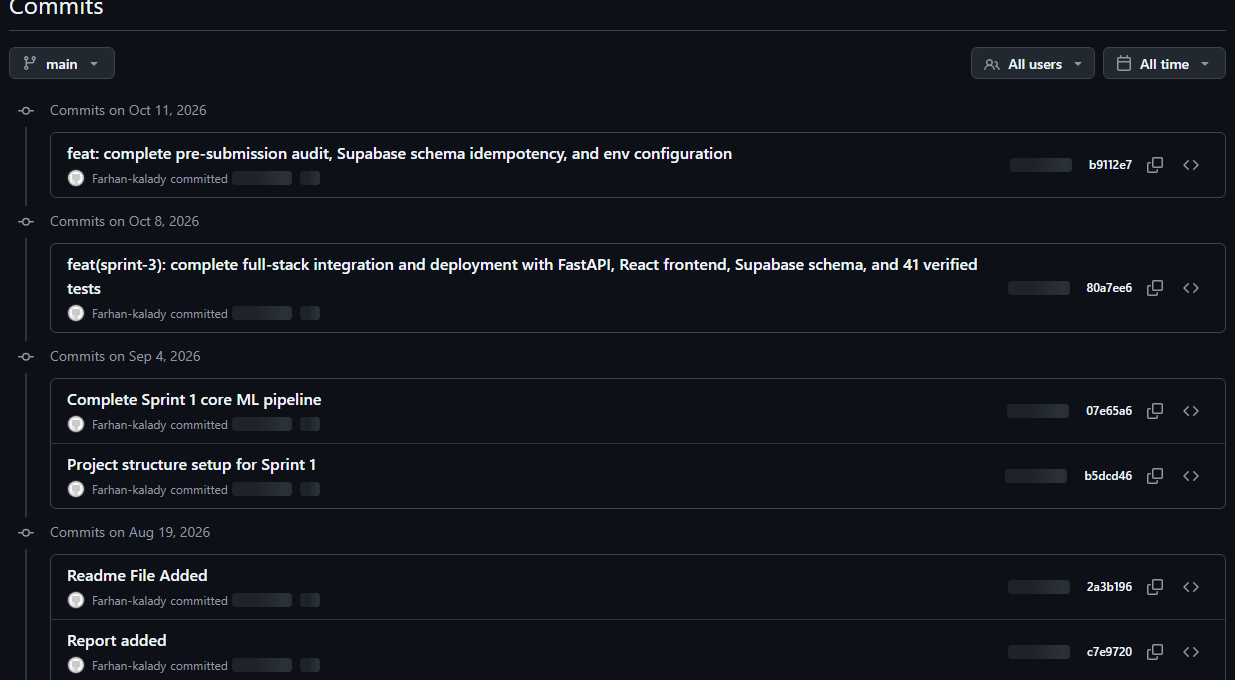
\includegraphics[width=0.96\textwidth]{figures/git_commit_history.png}
\caption{Verified GitHub repository commit history for ClauseIQ}\label{fig:github_commit_history}
\end{figure}

The source code and commit history are publicly accessible at the official repository: \url{https://github.com/Farhan-kalady/ClauseIQ.git}.

